\documentclass[paper=a4, fontsize=11pt]{scrartcl} % A4 paper and 11pt font size
\usepackage[T1]{fontenc} % Use 8-bit encoding that has 256 glyphs
\usepackage[english]{babel} % English language/hyphenation
\usepackage{multirow}
\usepackage{graphicx}
\usepackage{amsmath,amsfonts,amsthm} % Math packages
\usepackage{sectsty} % Allows customizing section commands
\allsectionsfont{\centering \normalfont\scshape} % Make all sections centered, the default font and small caps

\usepackage{fancyhdr} % Custom headers and footers
\pagestyle{fancyplain} % Makes all pages in the document conform to the custom headers and footers
\fancyhead{} % No page header - if you want one, create it in the same way as the footers below
\fancyfoot[L]{} % Empty left footer
\fancyfoot[C]{} % Empty center footer
\fancyfoot[R]{\thepage} % Page numbering for right footer
\renewcommand{\headrulewidth}{0pt} % Remove header underlines
\renewcommand{\footrulewidth}{0pt} % Remove footer underlines
\setlength{\headheight}{13.6pt} % Customize the height of the header
\graphicspath{{../Plots/}}
%\numberwithin{equation}{section} % Number equations within sections (i.e. 1.1, 1.2, 2.1, 2.2 instead of 1, 2, 3, 4)
%\numberwithin{figure}{section} % Number figures within sections (i.e. 1.1, 1.2, 2.1, 2.2 instead of 1, 2, 3, 4)
%\numberwithin{table}{section} % Number tables within sections (i.e. 1.1, 1.2, 2.1, 2.2 instead of 1, 2, 3, 4)

%\setlength\parindent{0pt} % Removes all indentation from paragraphs - comment this line for an assignment with lots of text

\newcommand{\horrule}[1]{\rule{\linewidth}{#1}} % Create horizontal rule command with 1 argument of height

\title{	
\normalfont \normalsize 
\textsc{TMA4220 Numerical Solution of Differential Equations by element methods} \\ [25pt] % Your university, school and/or department name(s)
\horrule{0.5pt} \\[0.4cm] % Thin top horizontal rule
\huge Part 2: Vibration analysis \\ % The assignment title
\horrule{2pt} \\[0.5cm] % Thick bottom horizontal rule
}

\author{Candidate numbers} % Your name

\date{\normalsize\today} % Today's date or a custom date

\begin{document}
\maketitle

\section*{Abstract}

\section*{Introduction}
With the displacement of spatial points in $x_1$- and $x_2$-direction represented as
\begin{equation*}
\boldsymbol{u} = \begin{bmatrix}
u_1 \\ u_2
\end{bmatrix}
\end{equation*}
the strain on each point is
\begin{equation*}
\begin{bmatrix}
\varepsilon_{11} \\
\varepsilon_{22} \\
\varepsilon_{12}
\end{bmatrix}
=
\begin{bmatrix}
\frac{\partial u_1}{\partial x_1} \\
\frac{\partial u_2}{\partial x_2} \\
\frac{\partial u_1}{\partial x_2}+\frac{\partial u_2}{\partial x_1}
\end{bmatrix}
\end{equation*}
as many notes on linear elasticity will let you know.\footnote{Note however that this is the form usually called engineer strain.} 

The connection between the strain $\varepsilon$ and the stress $\sigma$ is
\begin{align*}
\begin{bmatrix}
\sigma_{11} \\ \sigma_{22} \\ \sigma_{12}
\end{bmatrix}
&= \frac{E}{1-\nu^2}\begin{bmatrix}
1 & \nu & 0 \\
\nu & 1 & 0 \\
0 & 0 & \frac{1-\nu}{2}
\end{bmatrix}
\begin{bmatrix}
\varepsilon_{11} \\ \varepsilon_{22} \\ \varepsilon_{12}
\end{bmatrix} \\
\boldsymbol{\sigma} &= C\boldsymbol{\varepsilon}
\end{align*}
where $E$ is the Young's modulus and $\nu$ is the Poisson's ratio. Young's modulus characterises the solid's stiffness, i.e. large $E$ means that you need a large force to deform the solid. Poisson's ratio  is the ratio between the strains in $x_1$- and $x_2$-direction when submitting the solid to a stress in only one of the directions. To clarify: Consider a stress in only the $x_1$-direction direction\footnote{$\sigma_{11}$ being the only stress different from zero.}, then $\nu>0$ will say that the solid contracts in the $x_2$-direction and elongates in the $x_1$-direction. Worth noting is that $\nu<0$ is possible, and some materials actually have this property. Weird.
During the course of this analysis we will let $E$ and $\nu$ completely describe a solid's properties. No stress or strain due to difference in temperature.

\subsection*{The equation and a variational formulation}
In continuum mechanics
\begin{equation}
\label{vibDiff}
\rho \ddot{\boldsymbol{u}} = \nabla \sigma(\boldsymbol{u})
\end{equation}
describes the spatial displacement due to internal stresses alone. It is the extension of Hook's law and Newton's second law into a continuous medium. So rather than total mass we look at mass density, here denoted $\rho$.

To eventually arrive at variational formulation of (\ref{vibDiff}) we should spend some time with the right hand side of this equation to better understand it. For that reason we will take a slight detour and start our journey by considering the equation
\begin{align}
\label{linEl}
\nabla \sigma(\boldsymbol{u}) &= - \boldsymbol{f} \\
\left[\frac{\partial}{\partial x_1},  \frac{\partial}{\partial x_2}\right]\begin{bmatrix}
\sigma_{11} & \sigma_{12} \\
\sigma_{12} & \sigma_{22}
\end{bmatrix} &= -[f_1,f_2] \notag
\end{align}
working on some domain $\Omega$,
together with some boundary conditions, which in its general form looks a little something like
\begin{align*}
\boldsymbol{u} &= \boldsymbol{g}, \quad \text{on } \partial \Omega_D \\
\sigma(\boldsymbol{u})\cdot \boldsymbol{\hat{n}} &= \boldsymbol{h}, \quad \text{on } \partial \Omega_N
\end{align*}

As is usual procedure when trying to derive a variational formulation, we multiply (\ref{linEl}) with some test function $\boldsymbol{v}\in V$, where the function space $V$ will be determined from what seems useful during the derivation. Then we integrate over the domain to get
\begin{equation}
\label{step1}
\int_{\Omega} (\nabla \sigma(\boldsymbol{u}))\cdot \boldsymbol{v}d\Omega = -\int_{\Omega}\boldsymbol{f}\cdot \boldsymbol{v} d\Omega .
\end{equation}
We aim at applying Green's formula to the left hand side, and since Green's formula states that
\begin{equation*}
\int_{\Omega}\nabla \cdot \boldsymbol{a}d\Omega = \int_{\partial \Omega} \boldsymbol{a}\cdot \boldsymbol{\hat{n}}dS 
\end{equation*}
we should come up with a good candidate for $\boldsymbol{a}$. A good guess seems to be $\boldsymbol{a} = \sigma(\boldsymbol{u})\boldsymbol{v}$. Now, this isn't exactly the form the integrand on the left in (\ref{step1}) takes, so we need to do some calculations and find a relation between the two. Disclaimer for the following calculation: It is long, tedious and not extremely easy to read. In addition, for convenience's sake we use the notation $\frac{\partial}{\partial x_i} = \partial_{x_i}$.
\begin{align*}
\nabla \cdot (\sigma(\boldsymbol{u})\boldsymbol{v}) &= \nabla \cdot \begin{bmatrix}
\sigma_{11}v_1 + \sigma_{12}v_2 \\
\sigma_{12}v_1 + \sigma_{22}v_2
\end{bmatrix}\\
&= \partial_{x_1}(\sigma_{11}v_1 + \sigma_{12}v_2) + \partial_{x_2}(\sigma_{12}v_1 + \sigma_{22}v_2) \\
&= v_1\partial_{x_1}\sigma_{11} + \sigma_{11}\partial_{x_1}v_1 + v_2\partial_{x_1}\sigma_{12} + \sigma_{12}\partial_{x1}v_2  \\
&+ v_1\partial_{x_2}\sigma_{12} + \sigma_{12}\partial_{x2}v_1 + v_2\partial_{x_2}\sigma_{22} + \sigma_{22}\partial_{x_2}v_2 .
\end{align*}
Up to this point we've just done a vector dot product and some differentiation using the product rule. Let's continue by rearranging the terms to
\begin{align*}
\nabla \cdot (\sigma(\boldsymbol{u})\boldsymbol{v})&= v_1(\partial_{x_1}\sigma_{11} + \partial_{x_2}\sigma_{12}) + v_2(\partial_{x_1}\sigma_{12} + \partial_{x_2}\sigma_{22}) \\
&+ \sigma_{11}\partial_{x_1}v_1 + \sigma_{12}(\partial_{x_2}v_1+\partial_{x_1}v_2)+\sigma_{22}\partial_{x_2}v_2 .
\end{align*}
We're definitely closing in on something. To make it even more easy on the eye we go back to the integrand on the left in (\ref{step1}) and see that
\begin{equation*}
(\nabla \sigma(\boldsymbol{u}))\cdot \boldsymbol{v} = v_1(\partial_{x_1}\sigma_{11} + \partial_{x_2}\sigma_{12}) + v_2(\partial_{x_1}\sigma_{12} + \partial_{x_2}\sigma_{22}),
\end{equation*}
which corresponds nicely with the first part of what we have after rearranging terms. The last part we deal with by looking back at how the strain vector was defined. Using these two things we end up with
\begin{equation}
\label{step2}
\nabla \cdot (\sigma(\boldsymbol{u})\boldsymbol{v}) = (\nabla \sigma(\boldsymbol{u}))\cdot \boldsymbol{v} + \boldsymbol{\varepsilon}(\boldsymbol{v})\cdot \boldsymbol{\sigma}(\boldsymbol{u}).
\end{equation}
The result of putting this into (\ref{step1}) is
\begin{equation*}
\int_{\Omega}\boldsymbol{\varepsilon}(\boldsymbol{v})\cdot \boldsymbol{\sigma}(\boldsymbol{u})d\Omega - \int_{\Omega}\nabla \cdot (\sigma(\boldsymbol{u})\boldsymbol{v})d\Omega = \int_{\Omega}\boldsymbol{f}\cdot \boldsymbol{v} d\Omega,
\end{equation*}
and we've put ourselves in position to employ Green's formula on the second term on the left hand side. What we end up with is
\begin{equation*}
\int_{\Omega}\boldsymbol{\varepsilon}(\boldsymbol{v})\cdot \boldsymbol{\sigma}(\boldsymbol{u})d\Omega = \int_{\Omega}\boldsymbol{f}\cdot \boldsymbol{v} d\Omega + \int_{\partial \Omega}(\sigma(\boldsymbol{u})\boldsymbol{v})\cdot\boldsymbol{\hat{n}}dS,
\end{equation*}
and can be further simplified by letting $V = H^1_{\Gamma_D}=\{v \in H^1 : v=0$ on $\partial \Omega_D \}$. Then
\begin{align*}
\int_{\Omega}\boldsymbol{\varepsilon}(\boldsymbol{v})\cdot \boldsymbol{\sigma}(\boldsymbol{u})d\Omega &= \int_{\Omega}\boldsymbol{f}\cdot \boldsymbol{v} d\Omega + \int_{\partial \Omega_N}\boldsymbol{v}\cdot \sigma\boldsymbol{\hat{n}}dS  \notag \\
&= \int_{\Omega}\boldsymbol{f}\cdot \boldsymbol{v} d\Omega + \int_{\partial \Omega_N}\boldsymbol{v}\cdot\boldsymbol{h}dS
\end{align*}

We are now prepared to make a variational formulation of (\ref{linEl}): 

Find $u \in \{H^1 : u=g,$ on $\partial\Omega_D\}$ so that
\begin{equation}
\label{VarForm}
\int_{\Omega}\boldsymbol{\varepsilon}(\boldsymbol{v})\cdot C\boldsymbol{\varepsilon}(\boldsymbol{u})d\Omega = \int_{\Omega}\boldsymbol{f}\cdot \boldsymbol{v} d\Omega + \int_{\partial \Omega_N}\boldsymbol{v}\cdot\boldsymbol{h}dS
\end{equation}
for all $v\in V$. Here we have now substituted $C\boldsymbol{\varepsilon}$ for $\boldsymbol{\sigma}$.

\subsection*{Galerking projection}
Since both function spaces we're looking at er infinite dimensional it is a good idea to let the test function reside in the function space $X_h \subset V$ of piecewise linear functions on a triangulation of $\Omega$. Furthermore, let $X_h =$span$(\varphi_1,\ldots,\varphi_n)$ where $\varphi_i$ are basis function with some compact support. Since the test functions $v$ are now vector functions, there will for each node $\hat{i}$ be two test functions
\begin{align*}
\varphi_{\hat{i},1} &= \begin{bmatrix}
\varphi_{\hat{i}} \\ 0
\end{bmatrix} \\
\varphi_{\hat{i},2} &= \begin{bmatrix}
0 \\ \varphi_{\hat{i}}
\end{bmatrix},
\end{align*}
and there should be some connection between the basis number $i$, node number $\hat{i}$ and $d=1,2$. If the total number of nodes are $N$, then total number of basis functions should be $2N$. A good function between the two can be $i = 2\hat{i}+ (d-2)$. Then $i$ ranges from $1$ to $2N$. To build up a linear system of what we have so far we state the Galerkin formulation of the problem: Find $u \in X_h$ so that
\begin{equation}
\label{Galerkin}
\int_{\Omega}\boldsymbol{\varepsilon}(\boldsymbol{v})\cdot C\boldsymbol{\varepsilon}(\boldsymbol{u})d\Omega = \int_{\Omega}\boldsymbol{f}\cdot \boldsymbol{v} d\Omega + \int_{\partial \Omega_N}\boldsymbol{v}\cdot\boldsymbol{h}dS
\end{equation}
for all $v\in X_h$.

It is sufficient to find a $u$ where this is true for all the basis frunctions since the right hand side is a bilinear form and the right hand side is a linear functional. That means we can let $\boldsymbol{v} = \varphi_i$ with $i\in\{1,2,\ldots,2N\}$ and $u = \sum_j u_j\varphi_j$. We put this into our Galerking formulation as
\begin{align*}
\int_{\Omega}\boldsymbol{\varepsilon}(\boldsymbol{\varphi_i})\cdot C\boldsymbol{\varepsilon}\left(\sum_j u_j\boldsymbol{\varphi_j}\right)d\Omega &= \int_{\Omega}\sum_j u_j\boldsymbol{\varepsilon}(\boldsymbol{\varphi_i})\cdot C\boldsymbol{\varepsilon}(\boldsymbol{\varphi_j})d\Omega \\
&=\sum_j u_j\int_{\Omega}\boldsymbol{\varepsilon}(\boldsymbol{\varphi_i})\cdot C\boldsymbol{\varepsilon}(\boldsymbol{\varphi_j})d\Omega \\
&= \int_{\Omega}\boldsymbol{f}\cdot \boldsymbol{\varphi_i} d\Omega + \int_{\partial \Omega_N}\boldsymbol{\varphi_i}\cdot\boldsymbol{h}dS.
\end{align*}
Taking this to be true over all $i$ we get the linear system
\begin{equation*}
A\boldsymbol{u} = \boldsymbol{b},
\end{equation*}
where
\begin{align*}
A_{ij} &= \int_{\Omega}\boldsymbol{\varepsilon}(\boldsymbol{\varphi_i})\cdot C\boldsymbol{\varepsilon}(\boldsymbol{\varphi_j})d\Omega \\
b_i &=  \int_{\Omega}\boldsymbol{f}\cdot \boldsymbol{\varphi_i} d\Omega + \int_{\partial \Omega_N}\boldsymbol{\varphi_i}\cdot\boldsymbol{h}dS.
\end{align*}
This linear system is what we will be implementing.

\subsection*{A simple test case}
When using a finite element implementation it's in most cases a sound strategy to have compared to a test case where the exact solution is known. To build some confidence in the implementation. As a test example we are going to consider the following:
\begin{equation}
\label{testCase}
\begin{cases}\nabla \boldsymbol{\sigma}(\boldsymbol{u}) &= -\boldsymbol{f}, \quad \text{in } \Omega \\
\boldsymbol{u} &= \boldsymbol{0} \quad \text{on } \partial \Omega
\end{cases}
\end{equation}
where $\Omega = \{(x,y)\in \mathbb{R}^2: |x|,|y|<1\}$ and $\boldsymbol{f}$ is given as
\begin{align*}
f_1 &= \frac{E}{1-\nu^2}\left(-2y^2-x^2+\nu x^2-2\nu xy - 2xy + 3 - \nu\right) \\
f_2 &= \frac{E}{1-\nu^2}\left(-2x^2-y^2+\nu y^2-2\nu xy - 2xy + 3 - \nu\right).
\end{align*}
In addition we are given
\begin{equation*}
\boldsymbol{u} = \begin{bmatrix}
(x^2-1)(y^2-1) \\ (x^2-1)(y^2-1)
\end{bmatrix},
\end{equation*}
and all we need to do is verify that this is in fact the solution of (\ref{testCase}). So let's do just that. To begin with we notice easily that the boundary condition is satisfied, so we proceed by calculating the strains as
\begin{equation*}
\begin{bmatrix}
\varepsilon_{11} \\
\varepsilon_{22} \\
\varepsilon_{12}
\end{bmatrix}
=
\begin{bmatrix}
2x(y^2-1) \\
2y(x^2-1) \\
2y(x^2-1)+2x(y^2-1)
\end{bmatrix}.
\end{equation*}
Now we make use of the affine relation between $\sigma$ and $\varepsilon$ to deduce that
\begin{align*}
\begin{bmatrix}
\sigma_{11} \\
\sigma_{22} \\
\sigma_{12} \\
\end{bmatrix}
&= \frac{E}{1-\nu^2}\begin{bmatrix}
\varepsilon_{11} + \nu \varepsilon_{22} \\
\nu \varepsilon_{11} + \varepsilon_{22} \\
\frac{1-\nu}{2}\varepsilon_{12}
\end{bmatrix}
\\
&=\frac{E}{1-\nu^2}\begin{bmatrix}
2x(y^2-1) + 2\nu y(x^2-1) \\
2\nu x(y^2-1) +2y(x^2-1) \\
(1-\nu)(y(x^2-1)+x(y^2-1))
\end{bmatrix}
\end{align*} 
What follows is a tedious calculation, so brace yourself. The gradient of the stress is
\begin{align*}
\nabla \cdot \sigma(\boldsymbol{u}) &= \begin{bmatrix}
\partial_x \sigma_{11} + \partial_y \sigma_{12} \\
\partial_x \sigma_{12} + \partial_y \sigma_{22} 
\end{bmatrix} \\
&= \frac{E}{1-\nu^2}\begin{bmatrix}
2(y^2-1)+4\nu xy + (1-\nu)(x^2-1+2xy) \\
(1-\nu)(2xy + y^2-1)+4\nu xy +2(x^2 -1)
\end{bmatrix} \\
&= \frac{-E}{1-\nu^2}\begin{bmatrix}
-2y^2 - x^2 + \nu  x^2 - 2\nu xy - 2xy + 3 - \nu \\
-2x^2-y^2 + \nu y^2 - 2\nu xy -2xy + 3 -\nu
\end{bmatrix} \\
&= -\boldsymbol{f}
\end{align*}

So we now have a simple problem we know the analytic solution of and we can therefore use this to compare with what will become our finite element implementation.

\subsection*{Implementation in 2D}
Every implementation of the finite element method can roughly be separated into three steps: Preprocessing, solving the system and postprocessing the data. As for our test example given by (\ref{testCase}) the triangulated grid is given to us by the matlab script \textit{getPlate.m}, so the next step is constructing both stiffness matrix and the loading vector. As is standard procedure for finite element implementations we go through each element and calculate that element's contribution to both the stiffness matrix and loading vector.  Keep in mind that we are using triangular, linear elements, so every nodal basis function restricted to an element $T_k$ can be written $\varphi_{\hat{i}}\big|_{T_k} = c_0 + c_1x+c_2y$ for some coefficients $c_0,c_1$ and $c_2$. Furthermore, since we will restrict ourselves to using a Lagrangian nodal basis, the function evaluation of some basis function $\varphi_{\hat{i}}$ in the node $\textbf{x}_{\hat{j}}$ is $\varphi_{\hat{i}}(\textbf{x}_{\hat{j}}) = \delta_{\hat{i}\hat{j}}$\footnote{The Kronecker delta.}.

To determine these coefficients, let's say the domain of an element is the triangle with vertices $p_1, p_2$ and $p_3$, then the vector $[c_0, c_1, c_2]^T$ solves
\begin{equation*}
\begin{bmatrix}
1 & p_1^T \\
1 & p_2^T \\
1 & p_3^T
\end{bmatrix}
\begin{bmatrix}
c_0 \\ c_1 \\ c_2
\end{bmatrix}
= \begin{bmatrix}
1 \\ 0 \\ 0
\end{bmatrix}
\end{equation*}
if the vector corresponds to the coefficients of the basis function $\varphi\big|_{T_k}$ that is equal to $1$ in $p_1$. Notice that the right hand side is the first column vector of the three dimensional identity matrix. Similarly we can determine the coefficients of the basis function evaluating to one in the other points by using other column vectors of the identity matrix on the right hand side of the system.

Reiterating the our basis functions are vector valued (see the section on Galerking projection) we have that
\begin{equation*}
\boldsymbol{\varepsilon}\left(\varphi_{\hat{i},d}\right) = \begin{bmatrix}
c_1 \\ 0 \\ c_2
\end{bmatrix}
, \quad or \begin{bmatrix}
0 \\ c_2 \\ c_1
\end{bmatrix}
\end{equation*}
depending on whether $d=1$ or $2$ respectively. However, both these vectors are constant over the element's domain, and so the contribution of element $T_k$ to the stiffness matrix in row $i$, column $j$ is simply
\begin{equation*}
\boldsymbol{\varepsilon}(\varphi_i)\cdot C \boldsymbol{\varepsilon}(\varphi_j)\cdot \text{area}(T_k),
\end{equation*}
which is easily to compute.

As for the contributions to the loading vector the product $\varphi_i\cdot \boldsymbol{f}$ is not in general constant over any triangle, so we don't end up with as nice of a result as in the stiffness contribution case. To make ut simpler for ourselves we resort to using Gaussian quadrature. We use the same approach as for the stiffness matrix to determine the coefficients for the basis functions. Then simply taking the dot product of $\boldsymbol{f}$ and $\varphi_i$ to make a new function handler in the code, we are in a position to use the 2D numerical integrator we made in part 1 of this project.

So to sum up thus far: We go through each element on our global domain and calculate the coefficients of each basis function not vanishing on that element. Then we use these coefficients to calculate the contributions to the stiffness matrix and loading vector according to the above description. When this is done, the last thing we need to before solving the resulting system is to remove the rows and columns that corresponds to the Dirichlet boundary. After solving we put in $0$-values in the right place of the solution vector. See fig. \ref{fig:TestCase} for a comparison between the analytical and numerical solution of (\ref{testCase}).
\begin{figure}
\centering
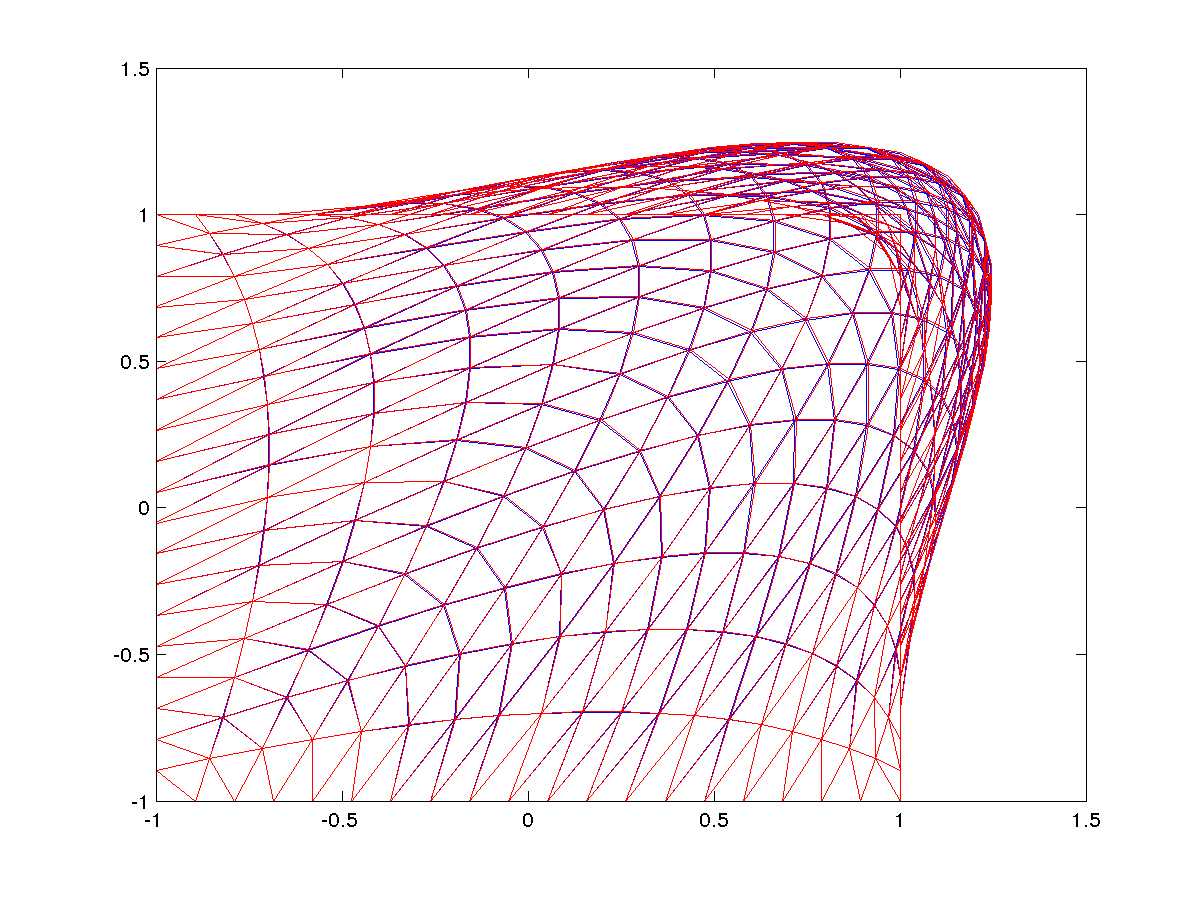
\includegraphics[scale=0.5]{Part2oppg2d20.png}
\label{fig:TestCase}
\caption{A comparison between the analytical and numerical solution of (\ref{testCase})}
\end{figure}
Instead of delving into analysing the error of our method we conclude from the figure that it seems to be working satisfactory.

\subsection*{Back to our main problem and moving up to 3D}
Finally we shall return to (\ref{vibDiff}) and consider a three-dimensional body. We have now that 
\begin{equation*}
\boldsymbol{\varepsilon} = 
\begin{bmatrix}
\varepsilon_{11} \\
\varepsilon_{22} \\
\varepsilon_{33} \\
\varepsilon_{12} \\
\varepsilon_{13} \\
\varepsilon_{23}
\end{bmatrix}
= \frac{1}{E}\begin{bmatrix}
1 & -\nu & -\nu & 0 & 0 & 0 \\
-\nu & 1 & -\nu & 0 & 0 & 0 \\
-\nu & -\nu & 1 & 0 & 0 & 0 \\
0 & 0 & 0 & 2(1+\nu) & 0 & 0 \\
0 & 0 & 0 & 0 & 2(1+\nu) & 0 \\
0 & 0 & 0 & 0 & 0 & 2(1+\nu)
\end{bmatrix}
\begin{bmatrix}
\sigma_{11} \\ \sigma_{22} \\ \sigma_{33} \\ \sigma_{12} \\ \sigma_{13} \\ \sigma_{23}
\end{bmatrix}
= C^{-1}\boldsymbol{\sigma},
\end{equation*}
 and so the stress-strain relation we will be using is $\boldsymbol{\sigma} = C\boldsymbol{\varepsilon}$ with
\begin{equation*}
C =
\begin{bmatrix}
\frac{E}{2\nu^2+\nu-1}\begin{bmatrix}
(\nu -1) & -\nu & -\nu \\
-\nu & (\nu-1) & -\nu \\
-\nu & -\nu & (\nu-1)
\end{bmatrix}
&
0_{3\times 3} \\
0_{3\times 3} &
\frac{E}{2(1+\nu)}I_{3\times 3}
\end{bmatrix},
\end{equation*}
where $0_{3\times 3}$ is to be read as a $3\times 3$-matrix consisting only of $0$-entries and $I_{3\times 3}$ is the $3\times 3$ identity matrix.

Using a very similar approach as in the 2D-case we have the variational formulation: Find $u\in V$ so that 
\begin{equation}
\rho \int_{\Omega}\boldsymbol{v}\cdot \boldsymbol{u}d\Omega=
-\int_{\Omega}\boldsymbol{\varepsilon}(\boldsymbol{v})\cdot C\boldsymbol{\varepsilon}(\boldsymbol{u})d\Omega
\label{newVar}
\end{equation}
for all $\boldsymbol{v}\in V$.

Again, rather than looking for a solution in the infinitely dimensional function space $V$ we let the test function reside in $X_h \subset V$. $X_h$ will be defined as before, only that now, since we are working in three dimensions,
\begin{equation*}
\varphi_{\hat{i},1} = \begin{bmatrix}
\varphi_{\hat{i}} \\ 0 \\ 0
\end{bmatrix}, \quad
\varphi_{\hat{i},2} = \begin{bmatrix}
 0 \\ \varphi_{\hat{i}}\\ 0
\end{bmatrix}, \quad
\varphi_{\hat{i},3} = \begin{bmatrix}
0 \\ 0 \\ \varphi_{\hat{i}}
\end{bmatrix}.
\end{equation*}
In addition the local-to-global function between the indices must now be rdefined to $i = 3\hat{i}+(d-3)$. With $N$ nodes we look for a solution of the form $u_h = \sum_{i=1}^{3N}u_{h,i}\varphi_i$ and say that (\ref{newVar}) must hold for all basis functions $\varphi_j$. What we end up with is the system
\begin{equation}
M\ddot{\boldsymbol{u}} = -A\boldsymbol{u}
\end{equation}
where
\begin{align*}
A_{ij} &= \int_\Omega \boldsymbol{\varepsilon}(\varphi_i)\cdot C\boldsymbol{\varepsilon}(\varphi_j)d\Omega  \\
M_{ij} &= \rho \int_{\Omega}\varphi_i \cdot \varphi_j d\Omega
\end{align*}
and the matrices are called the mass-- and stiffness matrix respectively.

The implementation of the stiffness matrix is the exact analogue of the 2D case and therefore doesn't need much of an elaboration. So let's spend a bit more time on one possible way of implementing the mass matrix $M$. As with the stiffness matrix we go through the domain $\Omega$ element by element and sum up the contributions. In contrast to how we calculated the contributions to loading vector we now transform the tetrahedral domain into a reference tetrahedron and calculate the contributions there. So consider an arbitrary tetrhedron $T_k$ with vertices $p_1, p_2, p_3$ and $p_4$. Then for any $x\in T_k$ the mapping
\begin{equation*}
\boldsymbol{\xi} = B(\boldsymbol{x}-p_1)
\end{equation*}
maps $\boldsymbol{x}=(x,y,z)^T$ to $\boldsymbol{\xi}=(\xi_1,\xi_2,\xi_3)^T$ which lies in the tetrahedron with vertices $(0,0,0)^T,(1,0,0)^T,(0,1,0)^T$ and $(0,0,1)^T$. Worth remarking on is that
\begin{equation}
A = \begin{bmatrix}
(p_2 - p_1) & (p_3-p_1) & (p_4-p_1)
\end{bmatrix}.
\end{equation} This tetrahedron we'll in the following call $S$ and it has has basis functions
\begin{align*}
\mathcal{H}_1(\boldsymbol{\xi}) = 1-\xi_1-\xi_2 - \xi_3 &\quad \mathcal{H}_2(\boldsymbol{\xi}) = \xi_1 \\
\mathcal{H}_3(\boldsymbol{\xi}) = \xi_2 &\quad \mathcal{H}_4(\boldsymbol{\xi}) = \xi_3.
\end{align*}
Notice now that the contribution to the mass matrix is
\begin{align*}
\int_{T_k}\rho \varphi_i(\boldsymbol{x})\cdot \varphi_j(\boldsymbol{x})d\Omega &= \int_{T_k}\rho \varphi_{\hat{i},d}(\boldsymbol{x})\cdot \varphi_{\hat{j},d}(\boldsymbol{x})d\Omega \\
&= \rho\cdot \text{det}(B)\int_S\mathcal{H}_{\alpha}(\boldsymbol{\xi})\mathcal{H}_{\beta}(\boldsymbol{\xi})dS.
\end{align*}
In the first equality we have taken advantage of the fact that $M_{ij}=0$ unless $\varphi_{\hat{i}}$ and $\varphi_{\hat{j}}$ are placed on the same element in the vector, i.e. when the $d$ in the local-to-global index mapping is the same for both $i$ and $j$. $\alpha, \beta = 1,2,3,4$ and corresponds to which of the vertices the original basis function should evaluate to one for. If we can calculate the mass matrix for the reference element $S$ we can use this to calculate the contributions. Let's call this mass matrix the prototype mass matrix and denote it $M_P$. The calculation isn't all that interesting so we just state the result, which is
\begin{equation*}
M_P = \frac{1}{60}\begin{bmatrix}
2 & 1 & 1 & 1 \\
1 & 2 & 1 & 1 \\
1 & 1 & 2 & 1 \\
1 & 1 & 1 & 2
\end{bmatrix}.
\end{equation*}
And so the elements contribution to M is simply
\begin{equation}
\rho\cdot \text{det}(A)
\end{equation}
\end{document}